\scanpage{53}
Supposons maintenant $k$ isomorphe à $\mathbf C$, et donnons nous une place pour laquelle $k$ est \uline{complet}. Alors \unsure{on a des réseaux|un des réseaux}
\diagram{\begin{tikzcd}[ampersand replacement=\&,column sep=small,row sep=0pt]
M_v^{\mathbf Z}\subset M^{\mathbb A_{\unsure{c|C}}}\quad\text{où}\quad M^{\mathbb A_{\unsure{c|C}}}=\deleted{\unsure{\mathbb A\otimes M}} \& \displaystyle\prod \& M(\ell) \\
\& |[draw,ellipse,inner sep=2pt]| {\substack{\ell\ \text{fini}\\\text{et }\uline{\text{infini}}}} \&
\end{tikzcd}}
est \unsure{indépendant}.

\deleted{On voit encore}

Si $M$ est défini sur \inserted{\figure{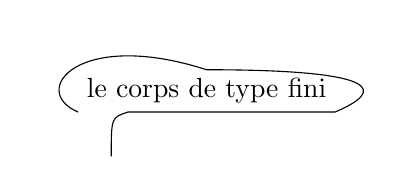
\begin{tikzpicture}[baseline=(n.base)]
\node[inner sep=3pt] (n) {le corps de type fini};
\draw (n.south west) .. controls ([xshift=-18pt]n.west) and ([yshift=15pt]n.north west) .. (n.north) .. controls ([xshift=18pt]n.north east) and ([xshift=18pt]n.east) .. (n.south east) -- ([xshift=18pt]n.south west) .. controls ([xshift=12pt,yshift=-2pt]n.south west) .. ([xshift=12pt,yshift=-16pt]n.south west);
\end{tikzpicture}}} $k_0$, et $k_0$ assez petit pour que $G_M$ connexe, mais \unsure{choisi} de degré de transcendance minimum, \deleted{alors si $\sigma\in\unsure{\operatorname{Aut}(k/k_0)}$ \unsure{tel que} $\sigma$ \unsure{de} \unsure{$M$} \unsure{fixe}} si $\sigma\in\deleted{\operatorname{Aut}_{k_0}k}\operatorname{Gal}(k/k_0)$
\margin{\figure{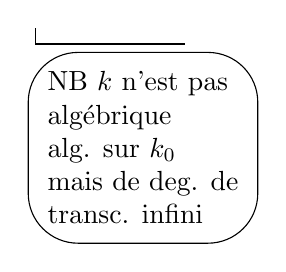
\begin{tikzpicture}
\draw (0.1,1.2)--(0.1,1)--(2,1);
\node[draw,rounded corners=18pt,align=left,inner sep=7pt,anchor=north west] at (0,0.9) {\uline{NB} $k$ n'est \uline{pas}\\\deleted{\unsure{algébrique}}\\\uline{alg. sur $k_0$}\\mais de deg. de\\transc. infini};
\end{tikzpicture}}}
on a
\[
M_{\sigma v}^{\mathbf Z}=\dot\sigma M_v^{\mathbf Z}
\]
où $\dot\sigma$ opère sur $M^{\mathbb A_{\unsure{c|C}}}$ \deleted{\unsure{en vertu}} de la façon suivante \deleted{\unsure{son image}}
\[
\dot\sigma\bigl((x_\ell)_{\ell\ \text{fini}},x_\infty\bigr)=(\sigma_\ell x_\ell,\dot\sigma_\infty x_\infty)
\]
où $\sigma_\ell$ provient de l'hom canonique
\[
\operatorname{Gal}(k/k_0)\mathbin{\text{---}}G(\mathbf Z_\ell),
\]
et $\dot\sigma_\infty$ est l'hom \uline{$\frac12$ linéaire} défini par $\sigma$ via
\[
\unsure{M_k|M_{/k}}(\infty)\simeq M_{k_0}(\infty)\otimes_{k_0}k.
\]
\mspage{52}
